\let\negmedspace\undefined
\let\negthickspace\undefined
\documentclass[journal]{IEEEtran}
\usepackage[a5paper, margin=10mm, onecolumn]{geometry}
%\usepackage{lmodern} % Ensure lmodern is loaded for pdflatex
\usepackage{tfrupee} % Include tfrupee package

\setlength{\headheight}{1cm} % Set the height of the header box
\setlength{\headsep}{0mm}     % Set the distance between the header box and the top of the text

\usepackage{gvv-book}
\usepackage{gvv}
\usepackage{cite}
\usepackage{amsmath,amssymb,amsfonts,amsthm}
\usepackage{algorithmic}
\usepackage{graphicx}
\usepackage{textcomp}
\usepackage{xcolor}
\usepackage{txfonts}
\usepackage{listings}
\usepackage{enumitem}
\usepackage{mathtools}
\usepackage{gensymb}
\usepackage{comment}
\usepackage[breaklinks=true]{hyperref}
\usepackage{tkz-euclide} 
\usepackage{listings}
% \usepackage{gvv}                                        
\def\inputGnumericTable{}                                 
\usepackage[latin1]{inputenc}                                
\usepackage{color}                                            
\usepackage{array}                                            
\usepackage{longtable}                                       
\usepackage{calc}  
\usepackage{amsmath,amssymb}

\usepackage{multicol}                                         
\usepackage{hhline}                                           
\usepackage{ifthen}                                           
\usepackage{lscape}
\begin{document}

\bibliographystyle{IEEEtran}

\title{
%	\logo{
NCERT - 9.5.10

\large{EE1003}
%	}
}
\author{Homa Harshitha Vuddanti

(EE24BTECH11062)
}	

\maketitle

\bigskip

\renewcommand{\thefigure}{\theenumi}
\renewcommand{\thetable}{\theenumi}
\textbf{Question}: Find a general solution of the differential equation
$\brak{x+y}\frac{dy}{dx}=1$\\
\textbf{Theoretical Solution:} \\
rearranging, we get $\frac{dx}{dy}-y=x$, \\
solving this as linear differential equation of first order by taking Integrating factor as\\
\begin{align}
e^{\int -1 \, dy}\\
e^{-y}
\end{align} We get the equation as 
\begin{align}
xe^{-y}=\int ye^{-y}dy +c
\end{align}
Solving this, we get 
\begin{align}
xe^{-y}=-(y+1)e^{-y}+c\\
x+y=ce^y-1
\end{align}
\textbf{Theoretical solution using Laplace transformation:}\\
The Laplace transformation of a function $f\brak{t}$ is
\begin{align}
\mathcal{L}\brak{f}=\int_{0}^{\infty} e^{-st}f\brak{t} dt=F\brak{s}
\end{align}
for the given differential equation 
\begin{align}
\brak{x+y}\frac{dy}{dx}=1 \label{eq:1}
\end{align}
let us take
\begin{align}
x+y=t
\end{align}
differentiating on both sides with respect to y,
\begin{align}
\frac{dx}{dy}+1=\frac{dt}{dy}\label{eq:2}
\end{align}
Substituting equation \eqref{eq:2} in \eqref{eq:1},
\begin{align}
\frac{dt}{dy}=t+1
\end{align}
Applying Laplace on both sides,
\begin{align}
\mathcal{L}\brak{t^\prime}=\mathcal{L}\brak{t+1}
\end{align}
Using the formula 
\begin{align}
\mathcal{L}\brak{f^\prime}=s\mathcal{L}\brak{f}-f\brak{0}\\
s\brak{T\brak{s}}-t\brak{0}=\frac{1}{s}+T\brak{s}\\
T\brak{s}=\frac{\frac{1}{s}+t\brak{0}}{s-1}
\end{align}
Applying inverse Laplace transformation,
\begin{align}
\mathcal{L}^{-1}\brak{T\brak{s}}=\mathcal{L}^{-1}\brak{\frac{1}{s\brak{s-1}}+\frac{t\brak{0}}{s-1}}\\
t=\brak{t\brak{0}+1}e^y -1\\
t=\brak{c}e^y-1
\end{align}
substituting $x+y=t$ we get final equation as
\begin{align}
x+y=ce^y-1
\end{align}
This is the same equation we obtained earlier.\\
\textbf{Theory:}
The derivative $\frac{dy}{dx}$ of a function $y=f\brak{x}$ is given by
\begin{align}
\frac{dy}{dx}=\lim_{h \to 0} \frac{f\brak{x+h}-f\brak{x}}{h}
\end{align}
Let us say \brak{x_0,y_0} are points that satisfy $f\brak{x}$, then 
\begin{align}
 \frac{dy}{dx}=\frac{y_1-y_0}{h}\\
  y_1=y_0+\frac{dy}{dx}h
\end{align}
Similarly,
\begin{align}
y_2=y_1+\frac{dy}{dx}h\\
y_{n+1}=y_n+h\frac{dy}{dx},\\
x_{n+1}=x_n+h
\end{align}
The difference equation will be of the form
\begin{align}
y_{n+1}=y_n+h\brak{\frac{1}{x_n+y_n}},\\
x_{n+1}=x_n+h
\end{align}

\textbf{Difference equation for $\frac{dx}{dy}$:}
This is similar to that of $\frac{dy}{dx}$ but the roles of $x$ and $y$ are reversed.
\begin{align}
\frac{dx}{dy}=\lim_{h \to 0} \frac{x\brak{y+h}-x\brak{y}}{h}\\
\frac{dx}{dy}=\frac{x_1-x_0}{h}\\
  x_1=x_0+\frac{dx}{dy}h,\\
  y_1=y_0+h
\end{align}
Thus the difference equation will become
\begin{align}
x_{n+1}=x_n+h\brak{x_n+y_n},\\
y_{n+1}=y_n+h
\end{align}
\textbf{Solving difference equation using one-sided z transformation:}
\begin{align}
X\brak{z}=\sum_{n=0}^{\infty} x\sbrak{n}z^{-n}
\end{align}
From difference equations,
\begin{align}
x_{n+1}-x_n&=h\brak{\frac{dx}{dy}}\\
y_{n+1}-y_n&=h
\end{align}
Applying one sided z transform on both sides,
\begin{align}
\mathcal{Z}\brak{x_{n+1}-x_n}&=\mathcal{Z}\brak{h\brak{\frac{dx}{dy}}}\\
\mathcal{Z}\brak{y_{n+1}-y_n}&=\mathcal{Z}\brak{h}
\end{align}
Applying the formula
\begin{align}
X\brak{z+1}&=zX\brak{z}-x_0,\\
zX\brak{z}-x_0-X\brak{z}&=\mathcal{Z}\brak{h\brak{x_n+y_n}}\\
zY\brak{z}-y_0-Y\brak{z}&=h\brak{\frac{1}{1-z^{-1}}}\\
Y\brak{z}&=\frac{y_0z^{-1}}{1-z^{-1}}+\frac{hz^{-1}}{1-z^{-1}}\\
X\brak{z}&=\frac{x_0+hY\brak{z}}{z-1-h}\\
X\brak{z}&=\frac{\brak{z^{-2}}\brak{h^2+hy_0\brak{1-z^{-1}}}}{\brak{1-z^{-1}-hz^{-1}}\brak{1-z^{-1}}^2}+\frac{x_0z^{-1}}{1-z^{-1}-hz^{-1}}\\
\end{align}
Splitting into partial fractions,
\begin{align}
X\brak{z}=\frac{z^{-1}\brak{-1-2h-y_0}}{1-z^{-1}}+\frac{-hz^{-2}}{\brak{1-z^{-1}}^2}+\frac{z^{-1}\brak{h^2+2h+y_0+x_0}}{1-z^{-1}-hz^{-1}}
\end{align}
\textbf{ROC:}
Casual ROC: $\abs{z}>\brak{1+h}$\\
Anti-casual ROC: $\abs{z}<1$\\
two sided ROC: $1<\abs{z}<\brak{1+h}$\\
Since we are considering $n\geq 0$, casual ROC can be taken.\\
Applying inverse z transform, 
\begin{align}
x_n&=\brak{h^2+2h+1+y_0+x_0}\brak{1+h}^n-\brak{1+2h+y_0+hn}\\
y_n&=y_0+nh
\end{align}
\textbf{Plotting:}
For this particular question, when we consider $c=0$, we get the equation as 
\begin{align}
y=-x-1
\end{align}
and a point \\
\begin{align}
\brak{x_0,y_0} = \brak{-1,0}
\end{align}
Using these, we can get points on the curve and plot it.\\
sim-1 is done using difference equation of $\frac{dy}{dx}$\\
sim-2 is done using difference equation of $\frac{dx}{dy}$\\
sim-3 is done using solving the difference equation by using one-sided z transformation
\begin{figure}[h!]
   \centering
   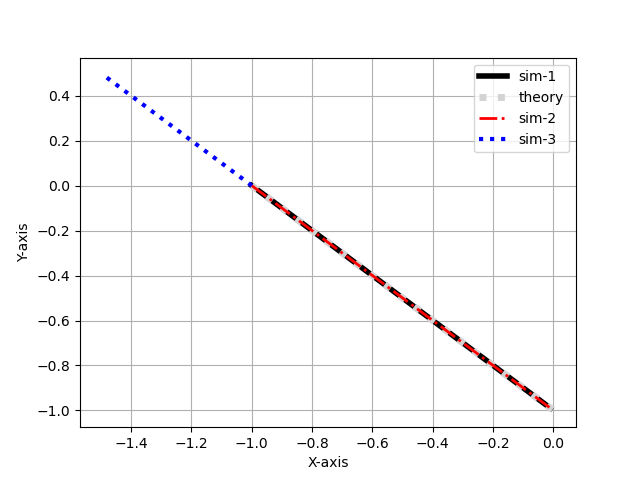
\includegraphics[width=1\columnwidth]{Figs/Figure_1.png}
   \caption{Plot}
\end{figure}
\end{document}
